\newpage
\section{Manuel utilisateur}
\label{sec:manuel}

\noindent Cette section est dédiée au manuel utilisateur. Ici, nous allons détailler les différentes actions, données dans \ref{sec:spec2} et \ref{sec:realisation}, sous la forme d'un guide pour l'utilisateur.

\subsection{Avant le match}

\paragraph{}
    Dans cette sous-section, nous allons détailler les différents écrans possible avant le match, avec des captures d'écrans légendes, pour expliquer les différentes actions possibles à l'utilisateur.

\begin{figure}[h]
\centering
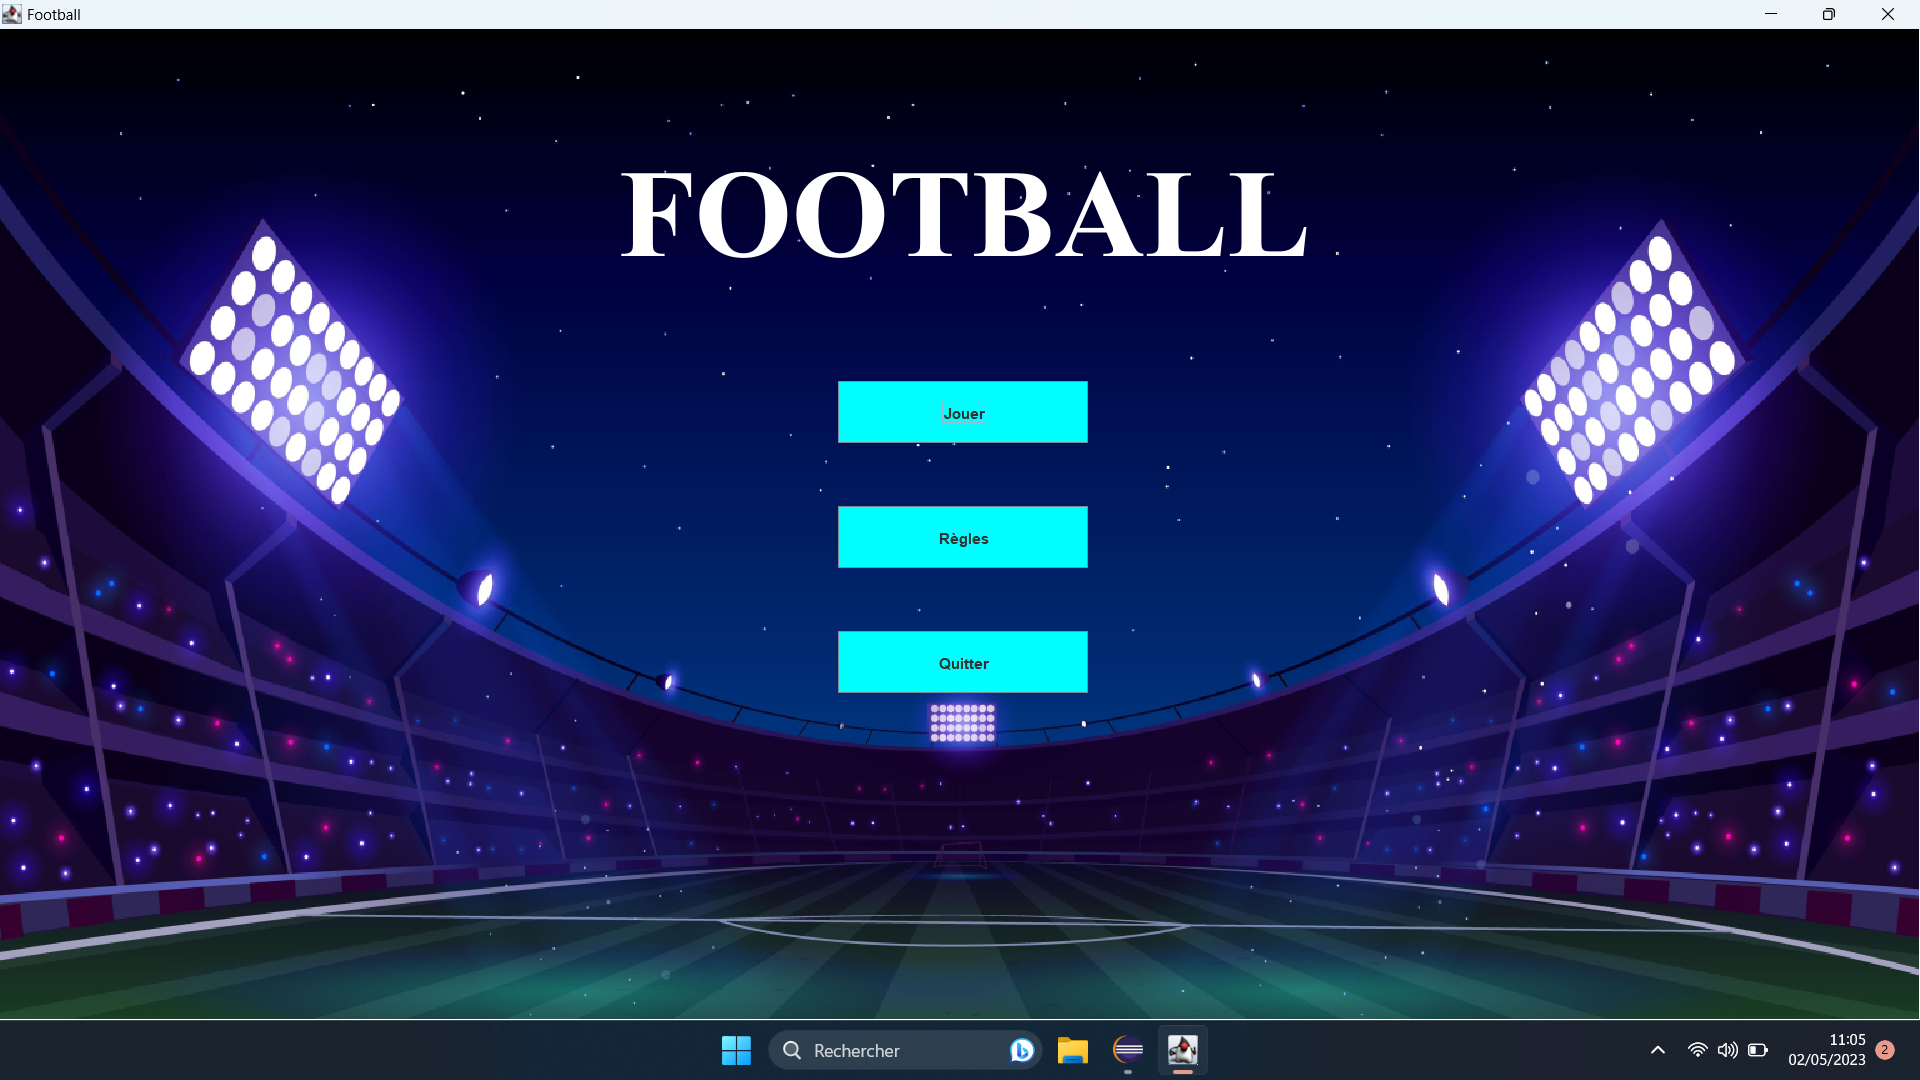
\includegraphics[width=12.82cm, height=8.2cm]{images/Accueil.png}
\caption{Page d'accueil}
\label{fig:accueil}
\end{figure}

\paragraph{Page d'accueil}


\begin{itemize}
    \item \textbf{Jouer :} 
        Si vous appuyez sur le bouton "Jouer" situé en haut, cela vous amènera à la page suivante qui est le choix d'équipe.

    \vspace{15pt}

    \item \textbf{Règles :} 
        Si vous appuyez sur le bouton "Règles" situé au milieu, cela vous amènera sur la page des règles du football.

    \vspace{15pt}

    \item \textbf{Quitter :} 
        Si vous appuyez sur le bouton "Quitter" situé en bas, cela vous fera quitter le jeu.
        
    \vspace{15pt}
\end{itemize}

\newpage

\begin{figure}[h]
\centering
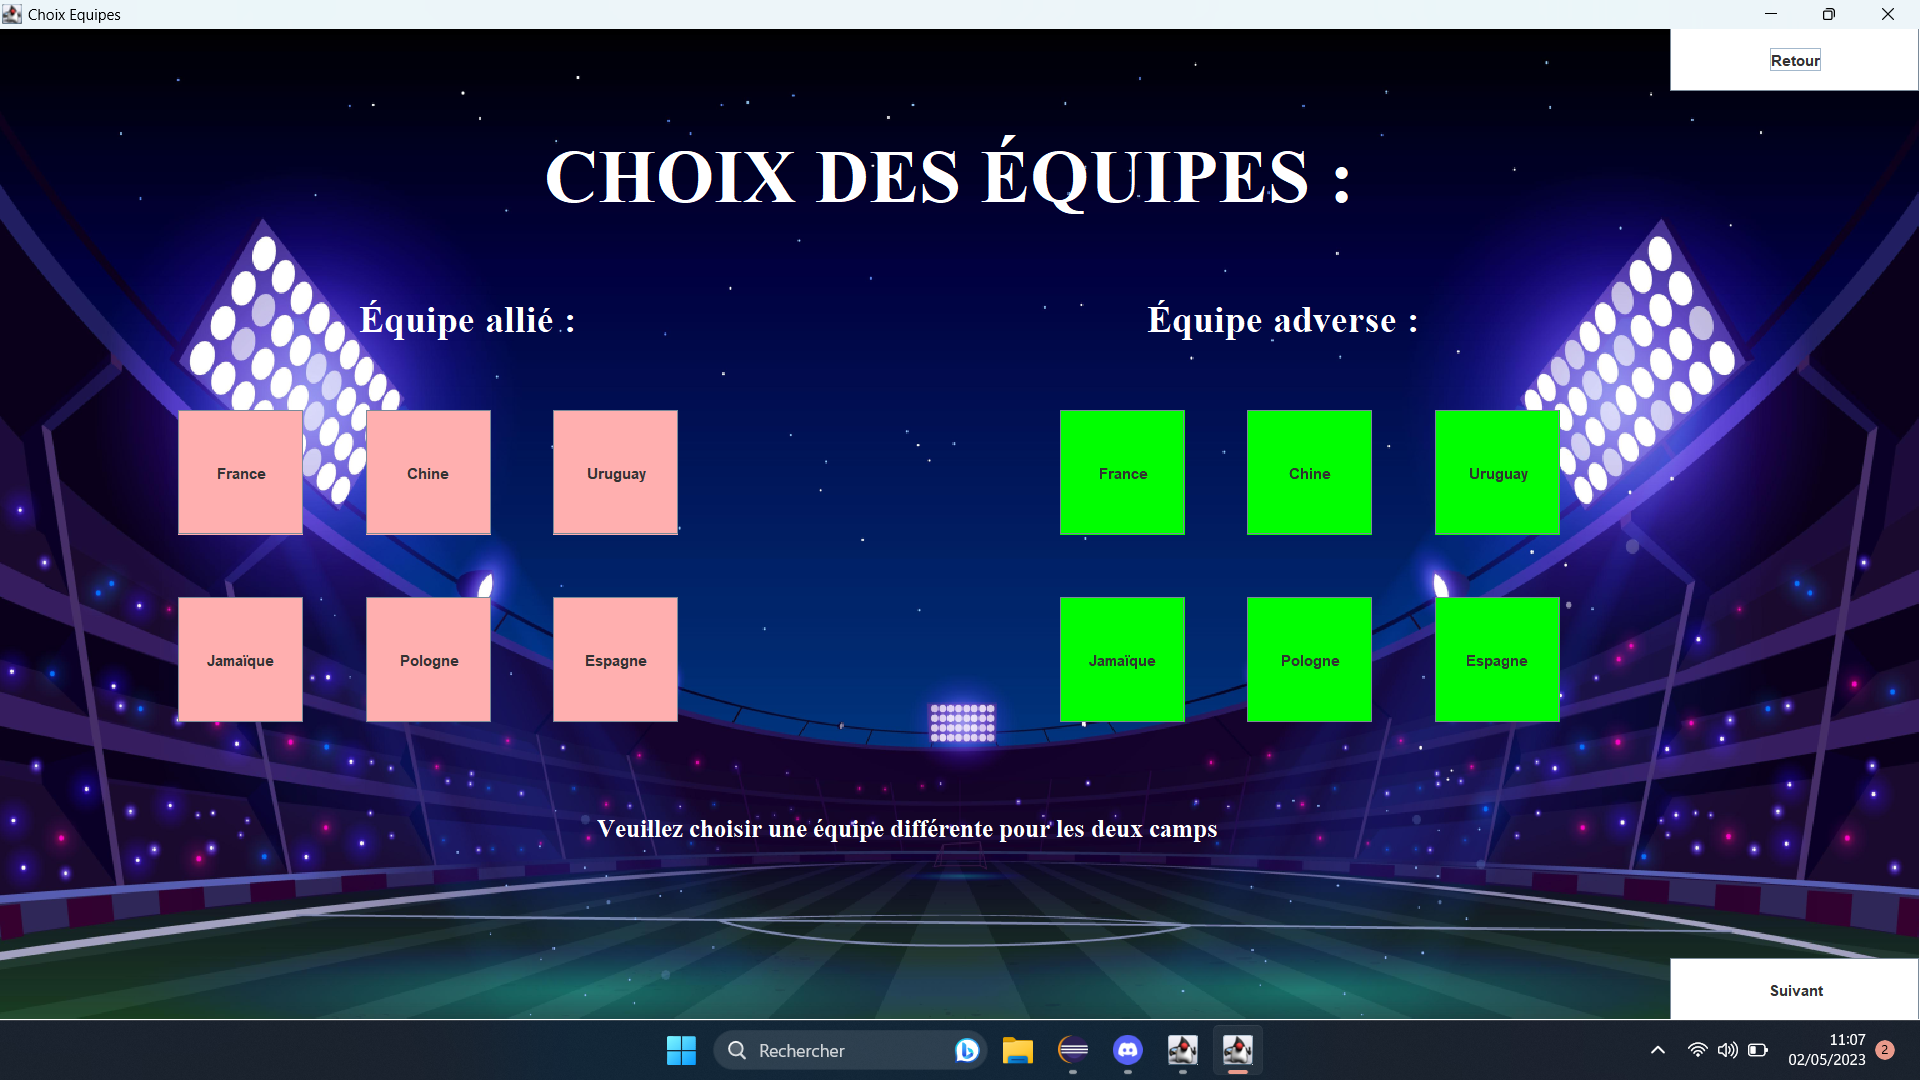
\includegraphics[width=12.82cm, height=8.2cm]{images/ChoixEquipe.png}
\caption{Choix Equipe}
\label{fig:choixEquipe}
\end{figure}

\paragraph{Page du choix des équipes}

\begin{itemize}
    \item \textbf{Retour :} 
        Si vous appuyez sur le bouton "Retour" situé en haut à droite, cela vous amènera à la page précédente qui est la page d'accueil.

    \vspace{15pt}

    \item \textbf{Les équipes :} 
        Au milieu de votre écran, vous voyez des noms de pays dans les cases roses et vertes, c'est ici que vous devez choisir le pays qui représentera votre équipe et celle de l'équipe adverse.

    \vspace{15pt}

    \item \textbf{Suivant :} 
        Si vous appuyez sur le bouton "Suivant" situé en bas à droite, cela vous amènera à la page suivante qui est la page de choix des postes, mais pour cela, vous devez choisir une équipe chacun.
        
    \vspace{15pt}
\end{itemize}

\begin{figure}[h]
\centering
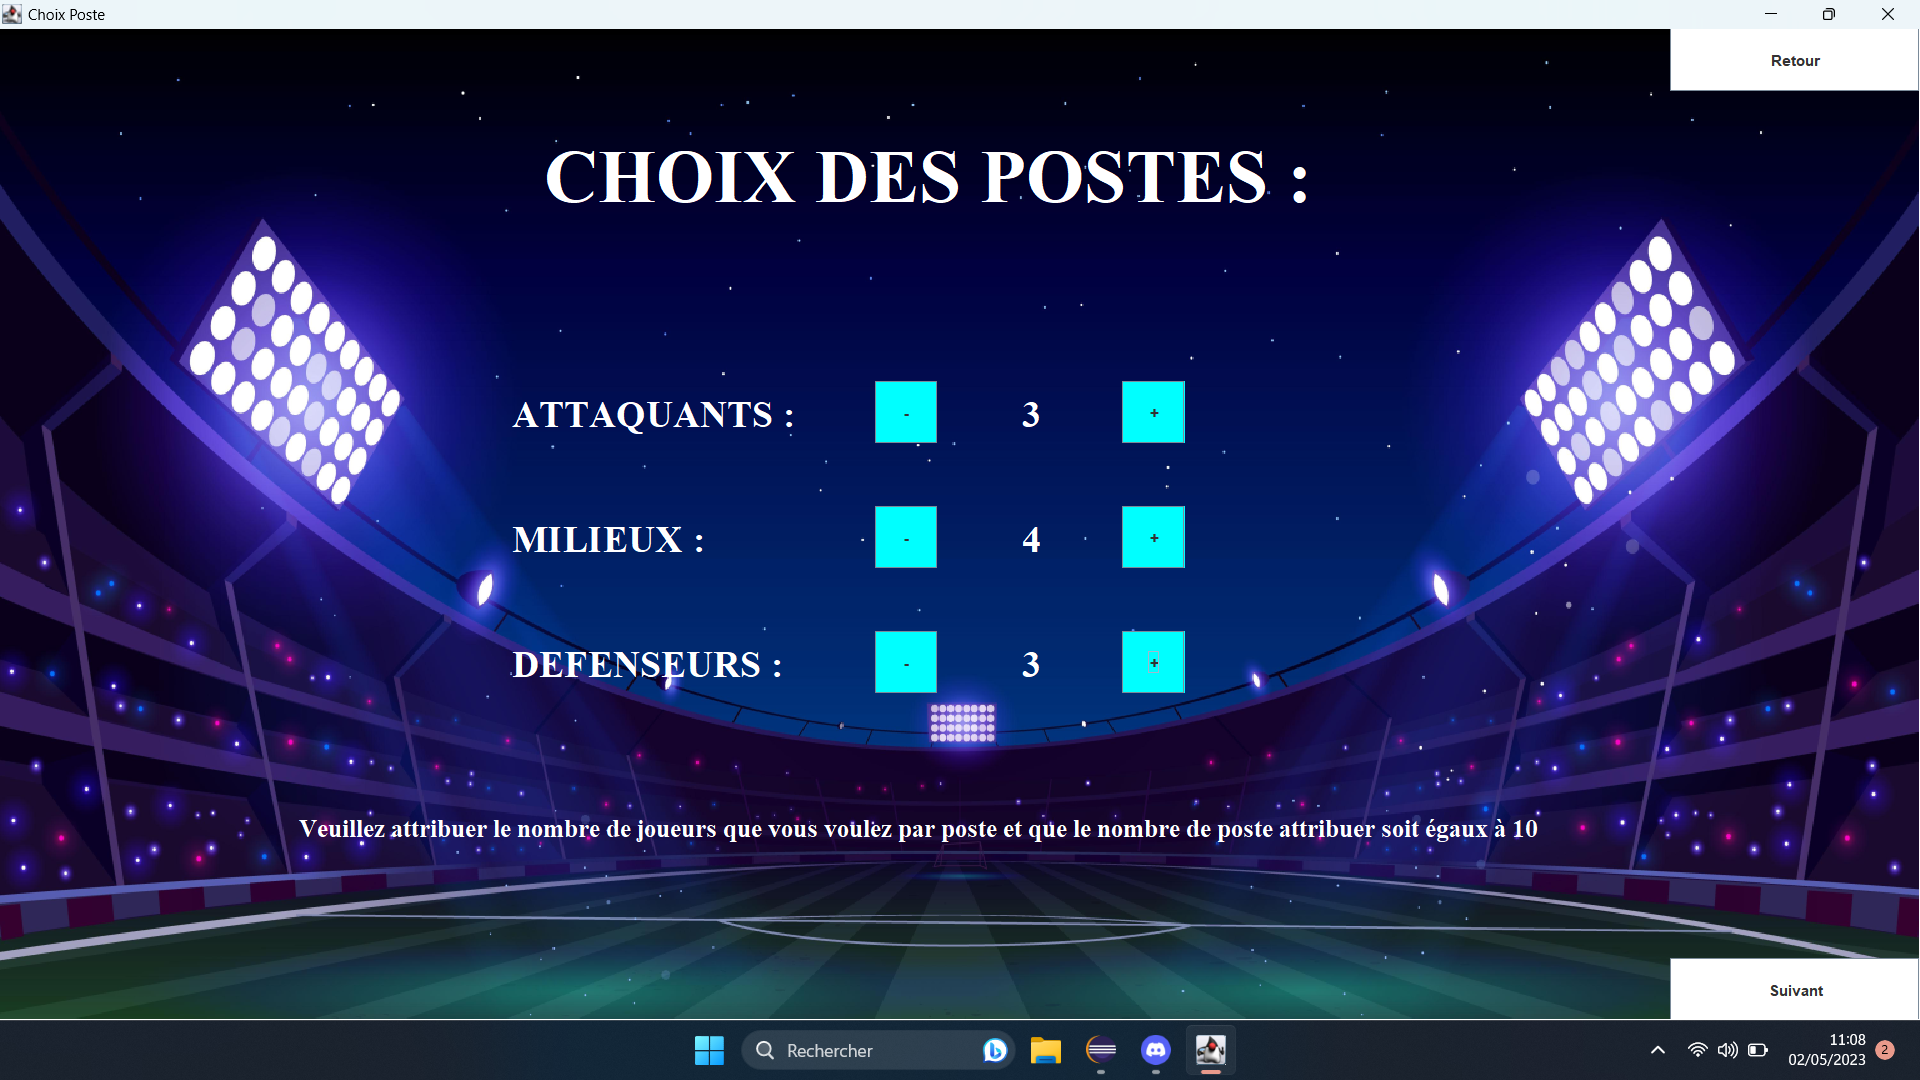
\includegraphics[width=12.82cm, height=8.2cm]{images/ChoixPoste.png}
\caption{Choix Poste}
\label{fig:choixPoste}
\end{figure}

    \vspace{15pt}

\paragraph{Page de la sélection de votre composition}

\begin{itemize}
    \item \textbf{Retour :} 
        Si vous appuyez sur le bouton "Retour" situé en haut à droite, cela vous amènera à la page précédente qui est la page de choix des équipes.

    \vspace{15pt}

    \item \textbf{Les postes :} 
        Au milieu de votre écran, vous voyez le nom des postes avec un bouton moins et plus, et au milieu un chiffre qui indique le nombre de personnes sur ce poste. Les boutons permettent d'ajouter ou d'enlever une personne à ce poste. Choisissez judicieusement votre composition, celle qui vous permettra d'obtenir la victoire.

    \vspace{15pt}

    \item \textbf{Suivant :} 
        Si vous appuyez sur le bouton "Suivant" situé en bas à droite, cela vous amènera à la page suivante qui est la page de choix des joueurs, mais pour cela, vous devez choisir 10 postes au total.
        
    \vspace{15pt}
\end{itemize}

\begin{figure}[h]
\centering
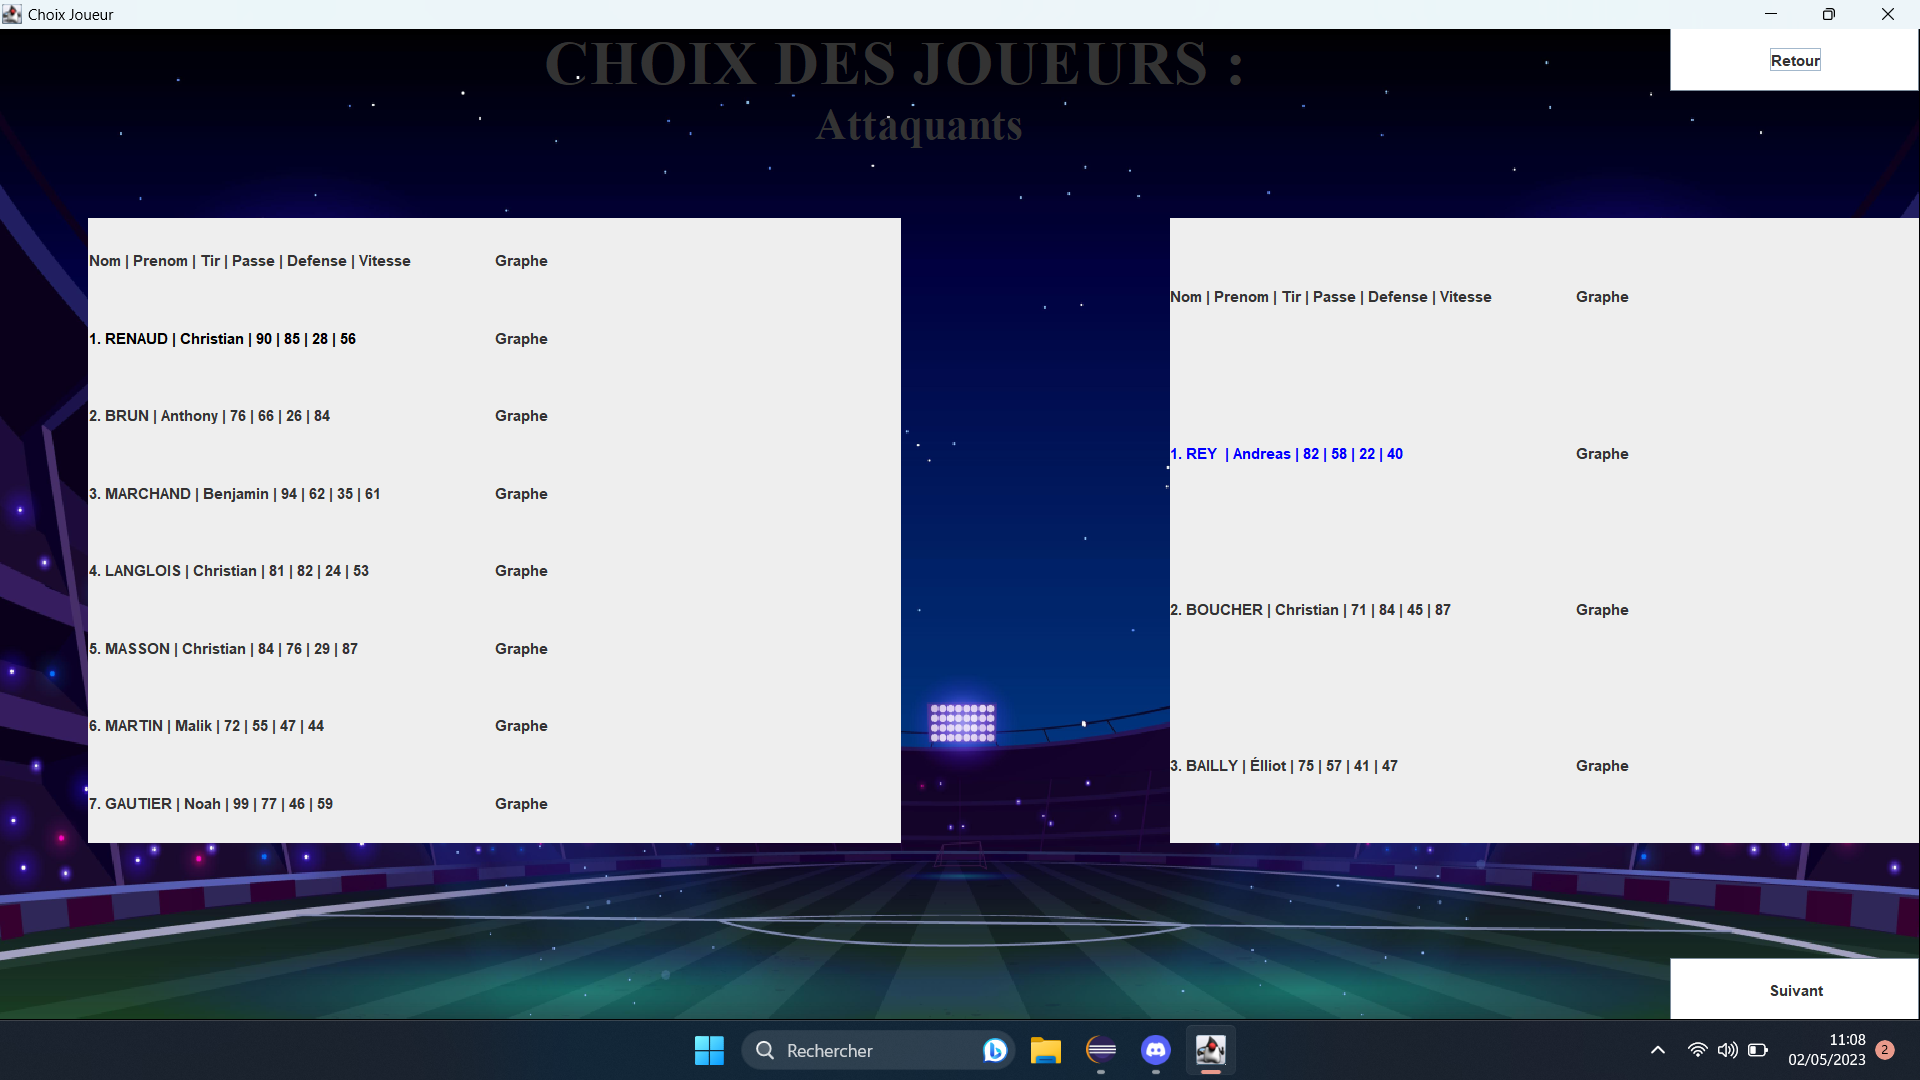
\includegraphics[width=12.82cm, height=8.2cm]{images/ChoixJoueur.png}
\caption{Choix Joueur}
\label{fig:choixJoueur}
\end{figure}

    \vspace{15pt}

\paragraph{Page de la sélection de vos joueurs}

\begin{itemize}
    \item \textbf{Retour :} 
        Si vous appuyez sur le bouton "Retour" situé en haut à droite, cela vous amènera à la page précédente qui est la page de choix des postes.

    \vspace{15pt}

    \item \textbf{Les joueurs :} 
         Au milieu de votre écran, vous voyez les joueurs avec leur nom, prénom et leurs statistiques liées à chacun. Vous devez choisir autant d'attaquants que de postes d'attaquant que vous avez choisis précédemment. Choisissez les meilleurs attaquants possible avec les meilleures statistiques possibles. Bien sûr, si vous vous êtes trompé d'attaquant, vous pouvez appuyer à nouveau dessus pour le faire partir.

    \vspace{15pt}

    \item \textbf{Suivant :} 
        Si vous appuyez sur le bouton "Suivant" situé en bas à droite, cela vous amènera à la page suivante qui est le match, mais pour cela, vous devez choisir le nombre d'attaquants que vous avez choisis. Ensuite, vous devez recommencer avec les milieux de terrain, puis les défenseurs et enfin le gardien.
        
    \vspace{15pt}
\end{itemize}















\subsection{Pendant le match}

\paragraph{}
    Dans cette sous-section, nous allons détailler les différentes actions qui seront réalisées durant le match, allant de la simulation d'un match de football aux statistiques calculées en temps réel, bien que l'utilisateur ne pourra rien faire étant donné que notre jeu n'est qu'une simulation.

\begin{figure}[h]
\centering
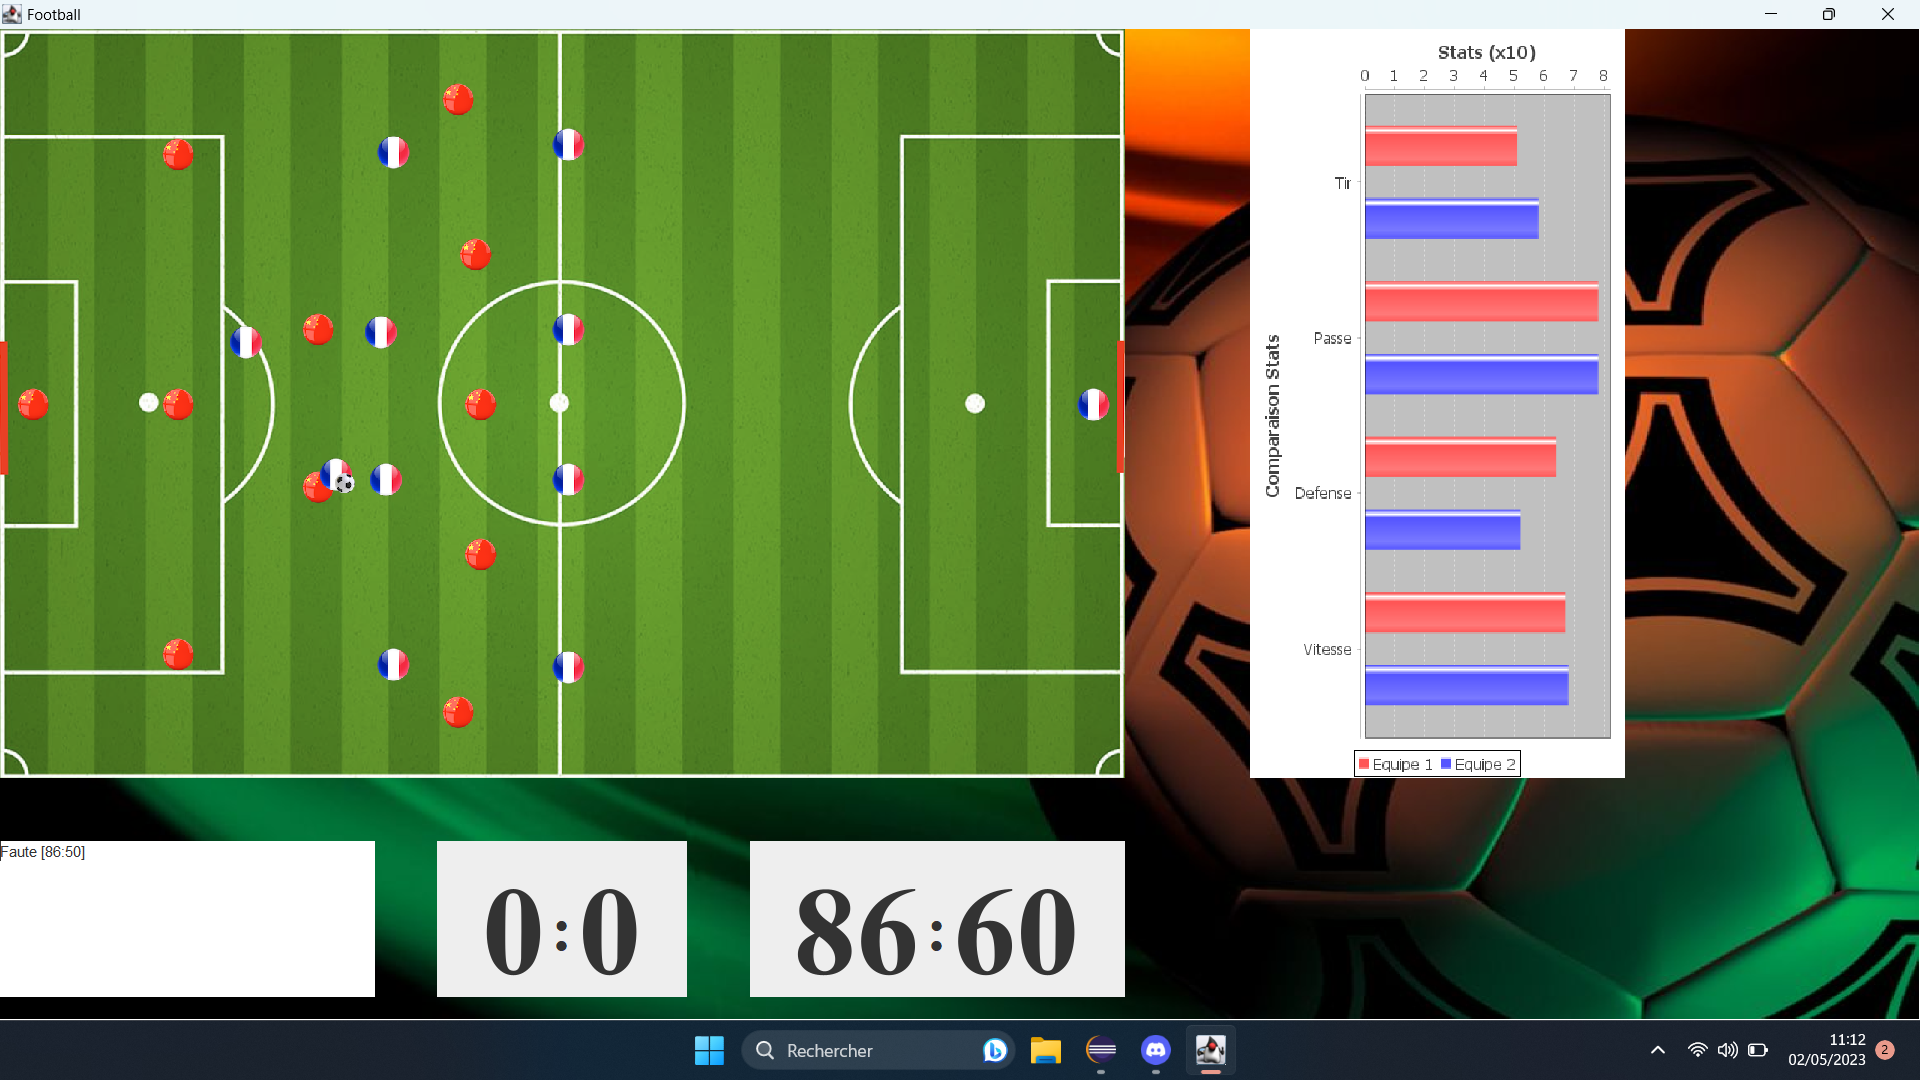
\includegraphics[width=12.82cm, height=8.2cm]{images/Match.png}
\caption{Match}
\label{fig:match}
\end{figure}

    \vspace{15pt}

\paragraph{Page de la simulation du match}

\begin{itemize}
    \item \textbf{En haut à gauche :} 
        Ceci est le match de football avec votre équipe positionnée à gauche et l'équipe adverse à droite. Maintenant, il ne vous reste plus qu'à regarder et encourager votre équipe. Bon match !

    \vspace{15pt}

    \item \textbf{À droite :} 
         Vous trouverez les moyennes des statistiques des joueurs en bleu pour votre équipe et en rouge pour l'équipe adverse à droite de votre écran.

    \vspace{15pt}

    \item \textbf{En bas} 
        \begin{itemize}
            
            \item \textbf{Les messages du jeux :}
                Le rectangle situé le plus à gauche est l'endroit où les actions spéciales telles que le corner, le but, etc., sont indiquées pour que vous puissiez suivre le match et comprendre ce qui se passe sans problème.
            
            \vspace{15pt}
            
            \item \textbf{Le score :}
                Le rectangle situé au milieu est l'endroit où les scores sont affichés. Ainsi, si votre équipe marque, vous pourrez le voir directement à cet endroit.

            \vspace{15pt}
            
            \item \textbf{Le temps :}
                Le rectangle à droite affiche le chronomètre pour vous permettre de savoir combien de temps il reste avant la fin du match. Lorsque le match est terminé, veuillez patienter 5 secondes et vous serez automatiquement redirigé vers la page des statistiques.
            
            \vspace{15pt}
        \end{itemize}

        
    \vspace{15pt}
\end{itemize}




    

\subsection{Après le match}

\paragraph{} 
    Dans cette sous-section, nous allons décrire l'affichage qui apparaîtra à la fin de la simulation de notre match de foot. Autrement dit, nous allons afficher les statistiques du match, le nom de l'équipe gagnante ainsi qu'un écran d'interaction avec l'utilisateur.

\begin{figure}[h]
\centering
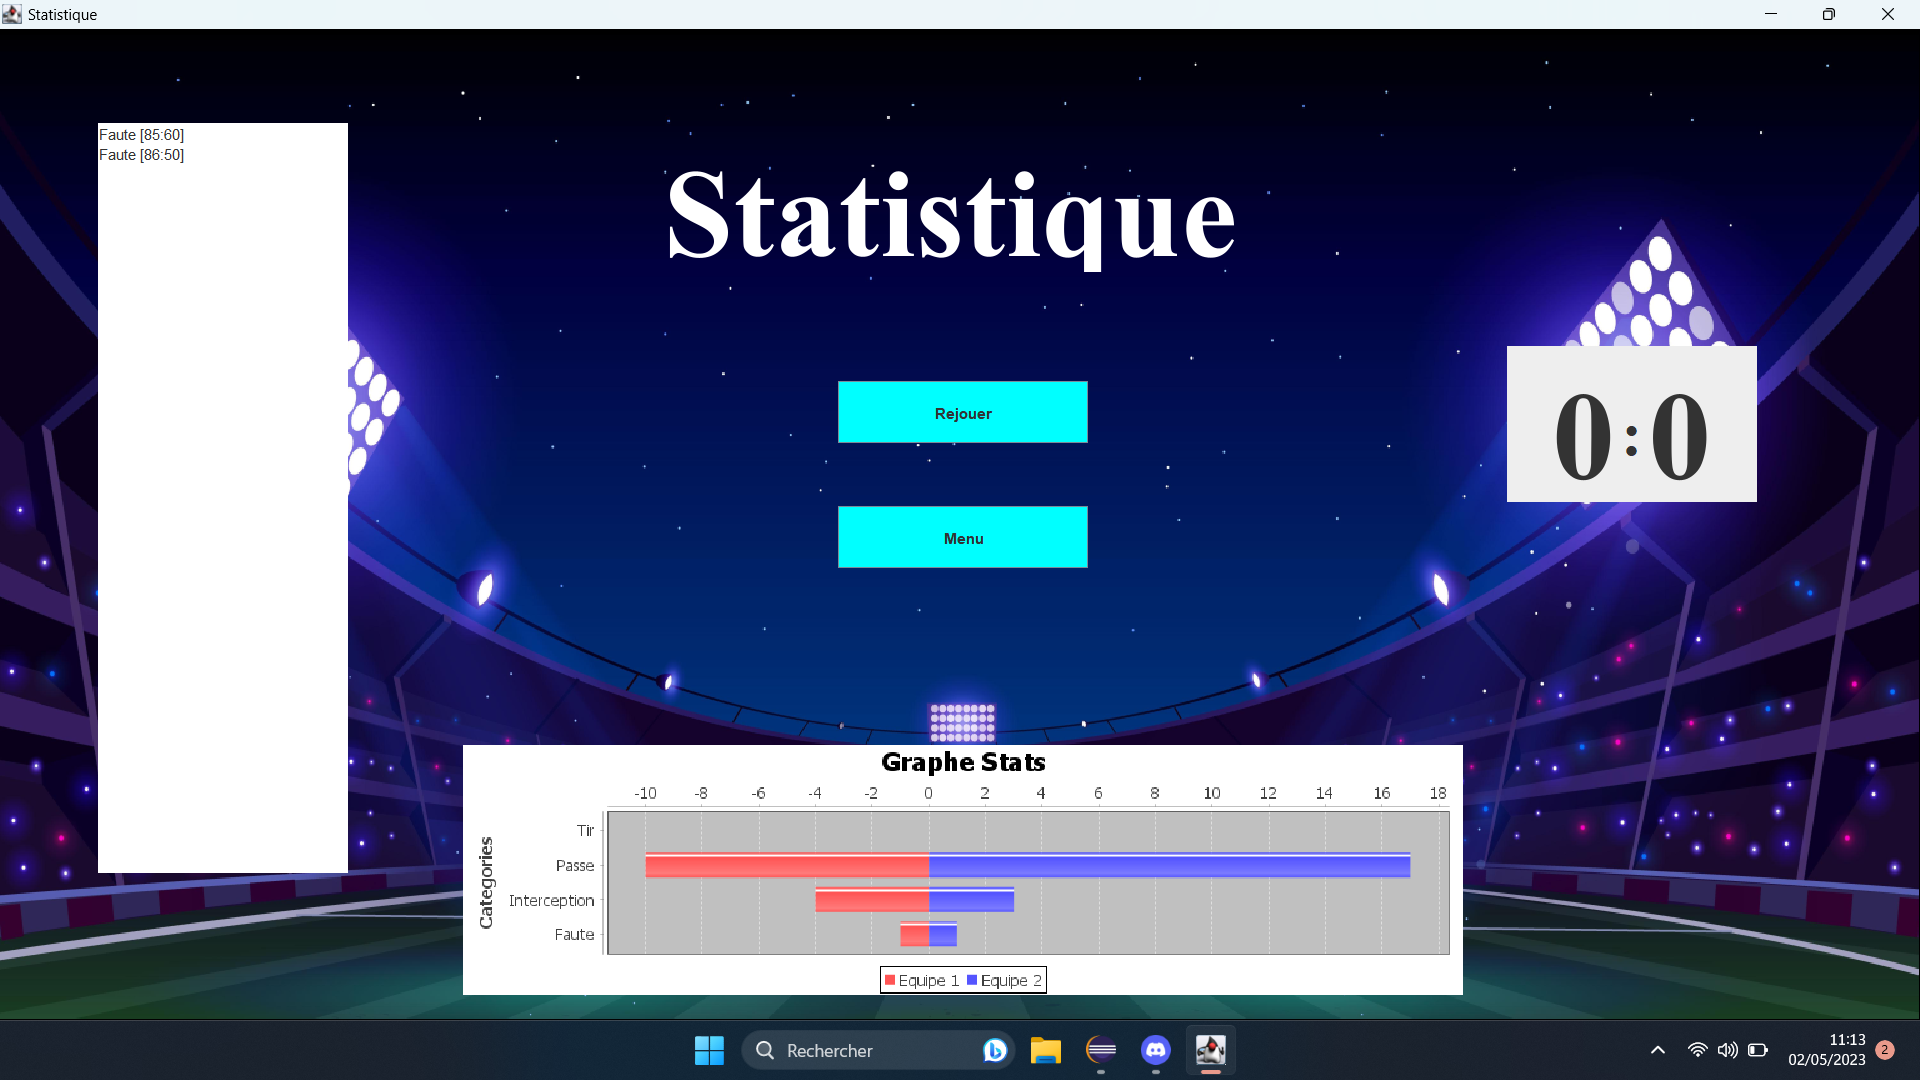
\includegraphics[width=12.82cm, height=8.2cm]{images/Statistiques.png}
\caption{Statistiques}
\label{fig:stats}
\end{figure}

    \vspace{15pt}

\paragraph{Page des statistiques}

\begin{itemize}
    \item \textbf{Rejouer :} 
        Si vous appuyez sur le bouton "Rejouer" il vous amènera directement sur la page du choix des équipes.

    \vspace{15pt}

    \item \textbf{Menu} 
         Si vous appuyez sur le bouton "Menu", cela vous amènera directement sur la page d'accueil.

    \vspace{15pt}

    \item \textbf{Les rectangles} 
        \begin{itemize}
            
            \item \textbf{Les messages du jeux :}
                Le rectangle situé à gauche est l'endroit où toutes les actions spéciales du match telles que le corner, le but, etc., sont indiquées afin que vous puissiez suivre le match et comprendre ce qui se passe sans problème.
            
            \vspace{15pt}
            
            \item \textbf{Le score :}
                Le rectangle situé à droite est l'endroit où les scores de fin de match sont affichés.

            \vspace{15pt}
            
            \item \textbf{Les statistiques}
                Le rectangle en bas affiche les statistiques de fin de match telles que le nombre de tirs, le nombre de passes, etc.
            
            \vspace{15pt}
        \end{itemize}
        
    \vspace{15pt}
\end{itemize}